\documentclass[10pt]{report}

% ============================================================
% PAGE SETUP
% ============================================================
% IEEE journal layout: narrow side margins, two columns 0.25 in apart
\usepackage[a4paper, top=0.75in, bottom=1in, left=0.625in, right=0.625in, columnsep=0.25in]{geometry}

% ============================================================
% CORE PACKAGES
% ============================================================
\usepackage[T1]{fontenc}
\usepackage[utf8]{inputenc}
\usepackage[australian]{babel}
\usepackage{textcomp}
\usepackage{graphicx}
\usepackage{float}
\usepackage{booktabs}
\usepackage{array}
\usepackage{tabularx}
\usepackage{amsmath}
\usepackage{mathtools}
\usepackage{newtxtext,newtxmath}   % Times, as in IEEE journals (after amsmath)
\usepackage[table]{xcolor}
\usepackage{tikz}
\usetikzlibrary{positioning, arrows.meta}   % needed for right=of / Stealth arrows
\usepackage{caption}
\usepackage{subcaption}
\usepackage{fancyhdr}
\usepackage{titlesec}
\usepackage{cite}
\usepackage{lettrine}
\usepackage[colorlinks=true, linkcolor=blue, citecolor=blue, urlcolor=blue]{hyperref}   % keep last

\graphicspath{{Images/}}

% Report figure: \reportfig{file.png} includes Images/file.png at column
% width, or draws a labelled box if the file has not been uploaded yet.
\newcommand{\reportfig}[2][\columnwidth]{%
    \IfFileExists{Images/#2}%
        {\includegraphics[width=#1]{Images/#2}}%
        {\fbox{\parbox[c][4cm][c]{0.9\columnwidth}{\centering\small Upload \texttt{Images/\detokenize{#2}}}}}}

% ============================================================
% COLOURS
% ============================================================
\definecolor{CoverGold}{RGB}{184,134,11}

% ============================================================
% SECTION FORMATTING
% ============================================================
% Use numbered \section{...} in each chapter file (not \section*),
% so the section counter steps and subsections restart at a. each time.
\renewcommand{\thesection}{\Roman{section}}
\renewcommand{\thesubsection}{\thesection-\Alph{subsection}}

% IEEE style: "I. Introduction" centred in small capitals, "A. Subsection" in italics
\titleformat{\section}{\centering\normalfont\normalsize\scshape}{\thesection.}{0.5em}{}
\titleformat{\subsection}{\normalfont\normalsize\itshape}{\Alph{subsection}.}{0.5em}{}
\titlespacing*{\section}{0pt}{1.0ex plus 0.2ex minus 0.2ex}{0.8ex}
\titlespacing*{\subsection}{0pt}{0.8ex plus 0.2ex minus 0.2ex}{0.5ex}

% ============================================================
% CAPTION FORMATTING
% ============================================================
\renewcommand{\tablename}{TABLE}
\renewcommand{\thetable}{\Roman{table}}
\captionsetup[table]{name=TABLE, position=above, justification=centering, singlelinecheck=false,
    font=footnotesize, labelfont=sc, textfont=sc, labelsep=newline, skip=4pt}
\captionsetup[figure]{name=Fig., position=below, justification=justified, singlelinecheck=true,
    font=footnotesize, labelsep=period, skip=4pt}

% ============================================================
% HEADER / FOOTER
% ============================================================
\pagestyle{fancy}
\fancyhf{}
\fancyfoot[C]{EGH446 Autonomous Systems \;|\; Semester 2, 2026 \;|\; \copyright\ QUT}
\fancyfoot[R]{\thepage}
\renewcommand{\headrulewidth}{0pt}

% ============================================================
% DOCUMENT
% ============================================================
\begin{document}

% No cover page: the title block at the top of 2_Introduction is the first
% page, as in an IEEE journal paper. (1_Cover_page.tex is kept but unused.)

% Each file below should open with a numbered section and a label:
%   2_Introduction        \section{INTRODUCTION}        \label{sec:intro}
%   3_Path_Planning       \section{PATH PLANNING}       \label{sec:planning}
%   4_Collision_Avoidance \section{COLLISION AVOIDANCE} \label{sec:avoidance}
%   5_Guidance_System     \section{GUIDANCE SYSTEM}     \label{sec:guidance}
%   6_Conclusion          \section{CONCLUSION}          \label{sec:conclusion}
%   7_References          \section*{REFERENCES}  (unnumbered)
% ============================================================
% TITLE BLOCK (spans both columns), ABSTRACT & INDEX TERMS
% ============================================================
% \tbd{...} marks values still to be filled in (prints red).
\providecommand{\tbd}[1]{\textcolor{red}{[#1]}}

\twocolumn[{%
    \centering
    {\huge Path Planning and Onboard Obstacle Avoidance for an\\[2pt]
    Autonomous Ground Robot among Unmapped Obstacles\par}
    \vspace{1.2em}
    {\large Chabod Masere, Jonah Menzies and Balin Carkeet\par}
    \vspace{0.4em}
    {\normalsize\itshape Group 50, School of Electrical Engineering and Robotics,
    Queensland University of Technology\par}
    \vspace{0.8em}
    {\footnotesize
    \begin{tabular}{@{}c c >{\centering\arraybackslash}m{0.5\textwidth} c@{}}
        \toprule
        \textbf{Name} & \textbf{Student no.} & \textbf{Contribution} & \textbf{Share} \\
        \midrule
        Chabod Masere & n10695141 & Collision avoidance design: re-planning and reactive layers, sensing & 33\% \\
        Jonah Menzies & n11395168 & Path planning: map inflation, A* routing, PSO smoothing, waypoint ordering & 33\% \\
        Balin Carkeet & n11336692 & Guidance: path following, waypoint capture and control & 33\% \\
        \bottomrule
    \end{tabular}\par}
    \vspace{1.6em}
}]

% Unnumbered first-page note, as on an IEEE first page
{\renewcommand{\thefootnote}{}\footnotetext{EGH446 Autonomous Systems, Major
Project Part~B. Submitted to the unit coordinator, Dr Luis Mejias, October 2026.}}

{\small\bfseries\emergencystretch=1em
\noindent\hspace{1em}\textit{Abstract}---This report presents the design and
evaluation of a navigation system that enables an autonomous ground robot to
visit a set of randomly generated waypoints in an arena containing obstacles
that are unknown in advance. Five waypoints are ordered using ant colony
optimisation over true driving distances, joined by an A* route on a map
inflated for clearance, and smoothed by particle swarm optimisation into a
path the vehicle can track. Twelve obstacles are detected only through onboard
sensing. When a detected obstacle lies near the remaining path, that part of
the path is re-planned around it, and a reactive potential field acts as a
close-range backup. Both layers are designed around a required clearance of
$0.40$~m, the vehicle radius plus a safety margin.
Across $25$ randomised missions the vehicle captured every waypoint,
completing a $108$~m mission in $117$~s on average. Measured from the
simulator's noise-free pose, it kept the required clearance in every
mission, with a margin of at least $0.20$~m: the closest passes were
$0.61$~m from an obstacle and $0.63$~m from a wall, and each waypoint
was passed within $0.24$~m. The estimator's
noise model was calibrated against the measured sensor noise, a
standard deviation of $0.10$~m and $2^{\circ}$, and the clearance
margins are sized against its measured error, $99$\% of which is below
$0.18$~m. Re-planning was essential: with it switched off, five of eight
test missions breached the clearance. A $1.5$~m/s speed limit was $26$\%
faster but left only $0.09$~m of margin, so $1.0$~m/s was kept.

\hspace{1em}\textit{Index Terms}---A* search, ant colony optimisation,
autonomous ground robots, configuration space, Kalman filter, noise
characterisation, obstacle avoidance, online re-planning, particle
swarm optimisation, path planning, potential field.
\par}
\vspace{0.6em}

% ============================================================
% INTRODUCTION
% ============================================================

\section{Introduction}
\label{sec:intro}

\lettrine{A}{utonomous} ground robots are increasingly deployed in
logistics, inspection, and industrial settings where they must travel
between goal locations without human intervention. To do this reliably,
a robot must know where it is, decide where to go next, and reach that
location without colliding with its surroundings.

Part~A of this project addressed the first two of these problems in an
obstacle-free field \cite{partA_est, partA_group}: the vehicle estimated
its state and drove straight between ordered waypoints. The subsystems
carried over from Part~A are summarised in Section~\ref{sec:guidance},
with the changes made for Part~B. Part~B adds
walls, which are known from a map, and obstacles, which are not known in
advance and can only be detected by onboard sensors as the vehicle
moves. This turns a tracking problem into a planning problem. The
waypoints must be ordered to keep the route short, a path must be found
around the walls, and that path must be revised whenever a sensor
reveals an obstacle on it.

\subsection{Task and System Overview}
\label{sec:overview}

The arena is a $52 \times 41$~m walled map containing twelve static
obstacles. The simulator treats an obstacle as a point; as the unit FAQ
(item 12) allows, each is taken to be a disc of radius $0.15$~m. The vehicle is an Ackermann-steered ground
robot of radius $0.25$~m that starts at $(2, 2)$~m. Each mission places
five waypoints at random in free space, at least $1.0$~m from every
obstacle's centre. The vehicle must visit all of them and stop on the last one,
keeping a margin of $0.15$~m between its body and every wall and
obstacle. Its centre must therefore stay at least
\begin{equation}
    d_{\text{clear}} = 0.25 + 0.15 = 0.40\ \text{m}
    \label{eq:clearance}
\end{equation}
from every wall face and obstacle surface. Throughout this report,
\emph{clearance} means this distance, from the vehicle's centre to a
wall face or an obstacle's surface, and the requirement is always
$0.40$~m. Where a distance is measured from an obstacle's centre
instead, it is stated as such: the requirement is then
$0.40 + 0.15 = 0.55$~m.

Figure~\ref{fig:architecture} shows the architecture and
Table~\ref{tab:io} the inputs, outputs and rate of each subsystem. During the mission
the state estimator supplies the state estimate
$\hat{\mathbf{x}} = [\hat{x}\ \hat{y}\ \hat{\theta}]^{\top}$, guidance
turns the path into a heading command, the reactive avoidance layer
adjusts it, and the controller converts it into speed and turn-rate
commands. The re-planner watches the object detector and replaces the
path when an obstacle is found near it.

Beyond the planning and avoidance methods taught in the unit, the
design adds four elements. (i) Waypoints are ordered by true driving
distance, the length of the A* route between each pair, not by
straight-line distance. (ii) Each A* leg is smoothed by PSO into a
B-spline that respects the vehicle's turning radius, with a fallback
that guarantees smoothing never reduces clearance. (iii) Obstacles are
remembered, filtered and confirmed before they are trusted, and the
re-planner tries a wider keep-out first, so that it routes around the
open side of an obstacle rather than through a gap beside a wall.
(iv) The estimator's noise model is measured from the simulator's
noise-free pose rather than assumed, and the planning and avoidance
margins are sized against the resulting estimate error. Each element is
compared with a simpler alternative in the sections that follow.

\begin{figure*}[t]
    \centering
    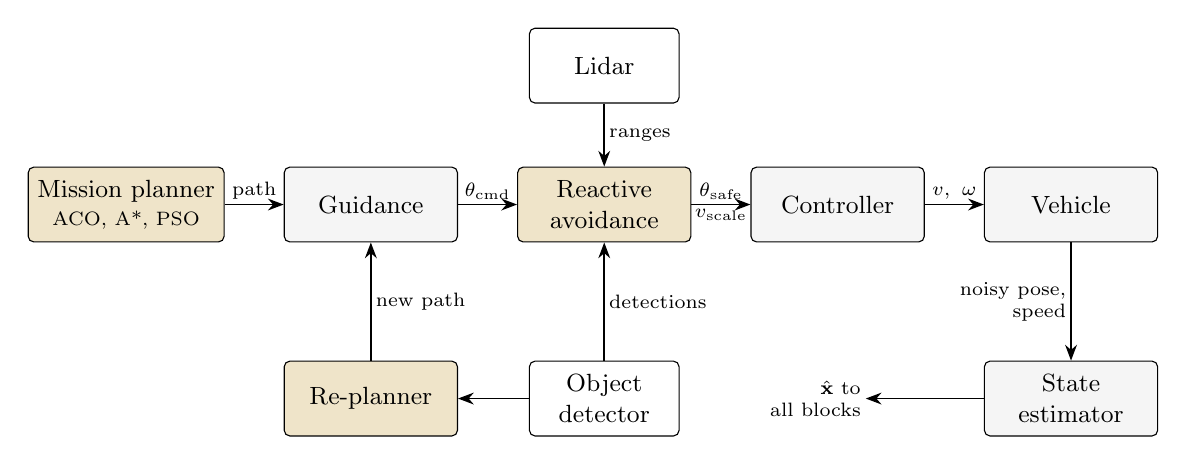
\begin{tikzpicture}[
        font=\small,
        node distance=0.9cm and 0.75cm,
        blk/.style={draw, rounded corners=2pt, minimum height=0.95cm,
                    minimum width=2.2cm, align=center, fill=black!4},
        new/.style={blk, fill=CoverGold!22},
        sen/.style={blk, minimum width=1.9cm, fill=white},
        arr/.style={-{Stealth[length=2mm]}, semithick},
        lab/.style={font=\scriptsize, inner sep=1.5pt}]

        % forward path
        \node[new] (plan) {Mission planner\\[-1pt]\scriptsize ACO, A*, PSO};
        \node[blk, right=of plan]  (guid) {Guidance};
        \node[new, right=of guid]  (avoid) {Reactive\\avoidance};
        \node[blk, right=of avoid] (ctrl) {Controller};
        \node[blk, right=of ctrl]  (veh)  {Vehicle};

        % feedback and sensing
        \node[blk, below=1.5cm of veh]   (est)  {State\\estimator};
        \node[new, below=1.5cm of guid]  (rep)  {Re-planner};
        \node[sen, below=1.5cm of avoid] (det)  {Object\\detector};
        \node[sen, above=0.8cm of avoid] (lid)  {Lidar};

        \draw[arr] (plan) -- node[lab, above] {path} (guid);
        \draw[arr] (guid) -- node[lab, above] {$\theta_{\text{cmd}}$} (avoid);
        \draw[arr] (avoid) -- node[lab, above] {$\theta_{\text{safe}}$}
                              node[lab, below] {$v_{\text{scale}}$} (ctrl);
        \draw[arr] (ctrl) -- node[lab, above] {$v,\ \omega$} (veh);

        \draw[arr] (veh) -- node[lab, left, align=right] {noisy pose,\\speed} (est);
        \draw[arr] (est.west) -- ++(-1.5,0)
              node[lab, left, align=right] {$\hat{\mathbf{x}}$ to\\all blocks};
        \draw[arr] (det) -- (rep);
        \draw[arr] (rep) -- node[lab, right] {new path} (guid);
        \draw[arr] (det) -- node[lab, right] {detections} (avoid);
        \draw[arr] (lid) -- node[lab, right] {ranges} (avoid);
    \end{tikzpicture}
    \caption{System architecture. Shaded blocks are new in Part~B. The
    state estimate $\hat{\mathbf{x}}$ is an input to guidance, reactive
    avoidance, the controller and the re-planner; those four connections
    are drawn as one arrow for clarity.}
    \label{fig:architecture}
\end{figure*}

\begin{table*}[t]
    \centering
    \caption{Subsystem Inputs and Outputs}
    \label{tab:io}
    \footnotesize
    \begin{tabularx}{\textwidth}{@{}l X X l@{}}
        \toprule
        \textbf{Subsystem} & \textbf{Inputs} & \textbf{Outputs} & \textbf{Rate} \\
        \midrule
        Mission planner    & Wall map, start pose, five waypoints & Waypoint order, path & Once, before the mission \\
        State estimator    & Noisy pose and speed & State estimate $\hat{\mathbf{x}}$ & 100 Hz \\
        Guidance           & Path, waypoint order, $\hat{\mathbf{x}}$ & Heading command $\theta_{\text{cmd}}$, distance to waypoint $d_{\text{wp}}$, waypoint index & 100 Hz \\
        Re-planner         & $\hat{\mathbf{x}}$, detections, waypoint index & Replacement path & 100 Hz; re-plans at most once per second \\
        Reactive avoidance & $\theta_{\text{cmd}}$, $\hat{\mathbf{x}}$, detections, lidar ranges, $d_{\text{wp}}$ & Safe heading $\theta_{\text{safe}}$, speed factor $v_{\text{scale}}$ & 100 Hz \\
        Controller         & $\theta_{\text{safe}}$, $\hat{\theta}$, $d_{\text{wp}}$, $v_{\text{scale}}$ & Speed $v$ and turn-rate $\omega$ commands & 100 Hz \\
        \bottomrule
    \end{tabularx}
\end{table*}

% ============================================================
% PATH PLANNING  (Requirement 4b)
% ============================================================
\section{Path Planning}
\label{sec:planning}

The planner runs once, before the vehicle moves, in five stages: inflate
the walls, route every pair of points with A* to obtain driving
distances, order the waypoints, route each leg in that order, and smooth
each leg with particle swarm optimisation (PSO). As the task requires,
it receives only the wall map and has no knowledge of the obstacles. The
obstacle list is read only when the random waypoints are drawn, to keep
them clear of obstacles; Fig.~\ref{fig:replan} shows a planned path
that runs inside the keep-out of an obstacle it did not know. Obstacles are
handled during the mission (Section~\ref{sec:avoidance}).

\subsection{Map Inflation}
Growing every wall by at least $d_{\text{clear}}$ lets the vehicle be planned as
a point in configuration space \cite{lozanoperez1983, lavalle2006}. The
map is an occupancy grid with $0.1$~m cells, and the planner searches
over the cell corners. Each wall cell is therefore first extended to the
four corners it touches, so that distances from those corners are true
distances from the wall faces. The walls are grown by $0.60$~m (six cells), not
$0.40$~m. The extra $0.20$~m is a tracking margin: the path is followed
from a noisy state estimate, and a path planned at exactly $0.40$~m
would breach the clearance with any tracking error.

\subsection{Working Principle}
\textbf{Routing.} Each leg is routed with A* \cite{hart1968} on the
inflated grid. A* expands the grid point with the lowest
\begin{equation}
    f(n) = g(n) + h(n),
    \label{eq:astar}
\end{equation}
where $g(n)$ is the path length from the start to point $n$ and $h(n)$
is the straight-line distance from $n$ to the goal. Points are
eight-connected. Because $h$ never overestimates the remaining distance,
the first path to reach the goal is the shortest one on the grid.

\textbf{Smoothing.} An A* path is made of straight runs joined at
$45^{\circ}$ corners and hugs the inflated walls (Fig.~\ref{fig:plan});
a steered vehicle cannot follow it. Each leg is therefore replaced by
a cubic B-spline whose control points start on the A* path, one per
metre, and may each move up to $1.0$~m sideways. A* fixes which way
round the walls a leg goes; PSO \cite{kennedy1995} only reshapes the
curve within that corridor. A particle is the vector of sideways
offsets, and the swarm minimises a cost evaluated along the curve,
\begin{equation}
\begin{aligned}
    J = \int \Big[\, 1 &+ k_{\kappa}\kappa^{2}
      + k_{t}\,\big(|\kappa| - \kappa_{\max}\big)_{+}^{2} \\
      &+ k_{s}\,\big(c_{s} - c\big)_{+}^{2}
      + k_{h}\,\big(c_{h} - c\big)_{+} \Big]\, ds,
\end{aligned}
\label{eq:psocost}
\end{equation}
where $s$ is arc length, so the first term is the path length, $\kappa$
is the curvature, $c$ is the distance to the nearest wall read from the
clearance field, and $(\cdot)_{+} = \max(0,\cdot)$. The second term
favours gentle curves, the third penalises any turn tighter than the
minimum radius, $\kappa_{\max} = 1/r_{\min}$ with $r_{\min} = 1.0$~m,
and the last two penalise coming within a soft clearance
$c_{s} = 0.90$~m of a wall and, far more heavily, within the hard
clearance $c_{h} = 0.60$~m. One particle starts with zero
offsets, so the A* path is always among the candidates, and a leg whose
best curve still breaches $c_{h}$ falls back to its A* path. Smoothing
can therefore never make a leg less safe than the route it started from.

\begin{figure}[!t]
    \centering
    \reportfig{fig_plan_k3.png}
    \caption{Planned mission: raw A* route and the planned path after PSO smoothing. Waypoints are
    numbered in visiting order.}
    \label{fig:plan}
\end{figure}

\subsection{Parameters}
The swarm uses $30$ particles for $150$ iterations per leg, with
inertia falling from $0.9$ to $0.4$ and acceleration weights of $1.5$,
and the cost weights are $k_{\kappa} = 1$, $k_{t} = 100$, $k_{s} = 20$
and $k_{h} = 10^{4}$, so that a breach of the hard clearance outweighs
every other term. The curvature limit follows from the controller limits of Section~\ref{sec:guidance}:
the tightest turn the vehicle can hold is the speed limit over the
turn-rate limit, $v_{\max}/\omega_{\max} = 0.80$~m, and $r_{\min} = 1.0$~m
leaves turn rate in reserve to correct tracking error during a turn.

\subsection{Advantages and Disadvantages}
A* is complete and optimal on the grid: if a route exists at the
required clearance it is found, and the same waypoints always give the
same route. Its weaknesses are that the path is only optimal to within
the eight grid directions, and that its cost grows with the number of
grid points, about $2.1 \times 10^{5}$ here. Building the distance
matrix took about $15$~s of the $17$~s planning time on a laptop.

PSO removes the first weakness. It needs no gradient, so the clearance
term is read straight from a lookup table, and it penalises turns
tighter than the vehicle can make: the sharpest point of each mission's
path had a curvature of $0.78$~m$^{-1}$ on average, and one leg of $125$
exceeded the limit of $1.0$~m$^{-1}$, by $1.4$\%. It is stochastic and gives no guarantee of a global
optimum, but both are contained by design: the $\pm 1.0$~m band keeps
every candidate in the corridor A* chose, and the fallback keeps the A*
leg when smoothing fails. Over the $125$ legs of
Section~\ref{sec:results} the fallback was never needed, and smoothing
shortened the path by $1.3$\% on average.

\subsection{Reasons for Choosing the Algorithm}
The walls are known and the map is small, so an exact grid search is
affordable and its guarantees are worth having. Dijkstra's algorithm
returns the same paths as A* but searches in every direction: on the
$40$ legs of missions $1$ to $8$ it expanded $3.7$ times as many grid
points for identical path lengths, which matters when fifteen pairs must
be routed. RRT and its optimal
variant RRT* \cite{karaman2011} are built for large or high-dimensional
spaces; in a two-dimensional arena with narrow doorways they are only
probabilistically complete, can miss a doorway with a finite number of
samples, and return a different route on every run. A* also gives the
true driving distance between any two points, which the waypoint
ordering needs. PSO was added because the corners of a raw A* path
demand a turn of zero radius, which the vehicle can only approximate by
cutting into the clearance margin.

\subsection{Waypoint Ordering}
The visiting order is found with the waypoint optimiser of Part~A
\cite{dorigo1997, partA_group}, unchanged except for its cost. In
Part~A the field was empty and the cost between two points was the
straight-line distance. Here two waypoints that are close together can be
separated by a wall, so the cost $D_{ij}$ is the length of the A* path
between points $i$ and $j$, the distance the vehicle must actually drive.
All fifteen pairs among the start and the five waypoints are routed to
build $D$, and the optimiser runs on $D$ as before. The change matters:
ordering by straight-line distance would have given a longer drive in
$13$ of the $25$ missions of Section~\ref{sec:results}, by $8.6$\% averaged
over all $25$ and up to $32$\%.

% ============================================================
% COLLISION AVOIDANCE  (Requirement 4c)
% ============================================================
\section{Collision Avoidance}
\label{sec:avoidance}

\subsection{Working Principle}
Obstacles are avoided in two layers (Fig.~\ref{fig:layers}). The first
is deliberative: when an obstacle is detected near the path still to be
driven, that part of the path is planned again around it. The second is
reactive: a potential field \cite{khatib1986} steers the vehicle away
from any obstacle whose centre comes within $0.8$~m. Re-planning does most of
the work because it acts early and keeps the guarantees of the planner;
the reactive layer covers what re-planning cannot, such as an obstacle
confirmed too late. Neither layer reads the obstacle list. Every
obstacle position they use comes from the onboard detector.

\begin{figure}[!t]
    \centering
    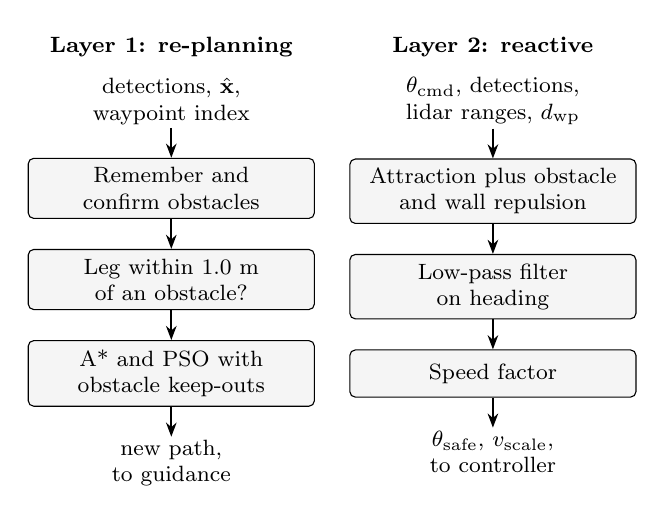
\begin{tikzpicture}[
        font=\footnotesize,
        node distance=0.38cm,
        io/.style={align=center, inner sep=1pt},
        st/.style={draw, rounded corners=2pt, minimum height=0.6cm,
                   text width=3.4cm, align=center, fill=black!4},
        arr/.style={-{Stealth[length=1.8mm]}, semithick}]
        % layer 1
        \node[io, text width=3.5cm] (i1) {detections, $\hat{\mathbf{x}}$,\\waypoint index};
        \node[st, below=of i1] (m)  {Remember and confirm obstacles};
        \node[st, below=of m]  (t)  {Leg within $1.0$~m\\of an obstacle?};
        \node[st, below=of t]  (r)  {A* and PSO with\\obstacle keep-outs};
        \node[io, below=of r, text width=3.5cm] (o1) {new path,\\to guidance};
        \draw[arr] (i1) -- (m);  \draw[arr] (m) -- (t);
        \draw[arr] (t) -- (r);   \draw[arr] (r) -- (o1);
        % layer 2
        \node[io, text width=3.5cm, right=0.5cm of i1] (i2) {$\theta_{\text{cmd}}$, detections,\\lidar ranges, $d_{\text{wp}}$};
        \node[st, below=of i2] (p)  {Attraction plus obstacle and wall repulsion};
        \node[st, below=of p]  (f)  {Low-pass filter\\on heading};
        \node[st, below=of f]  (s)  {Speed factor};
        \node[io, below=of s, text width=3.5cm] (o2) {$\theta_{\text{safe}}$, $v_{\text{scale}}$,\\to controller};
        \draw[arr] (i2) -- (p);  \draw[arr] (p) -- (f);
        \draw[arr] (f) -- (s);   \draw[arr] (s) -- (o2);
        \node[above=0.1cm of i1, font=\footnotesize\bfseries] {Layer 1: re-planning};
        \node[above=0.1cm of i2, font=\footnotesize\bfseries] {Layer 2: reactive};
    \end{tikzpicture}
    \caption{The two avoidance layers: inputs, stages and outputs.}
    \label{fig:layers}
\end{figure}

\textbf{Layer 1: online re-planning.} The re-planner runs at $100$~Hz.
\begin{enumerate}
    \item \textit{Remember.} Each detection is converted to a world
    position with Eq.~\eqref{eq:detection}. A detection within $0.75$~m
    of a known obstacle updates that obstacle's position with a
    first-order filter; any other starts a new obstacle.
    \item \textit{Confirm.} An obstacle is trusted once it has been
    seen on $20$ re-planner steps ($0.2$~s, two or three detector updates).
    \item \textit{Trigger.} A leg is re-planned if the part still to be
    driven passes within $1.0$~m of a confirmed obstacle's centre. Re-planning
    runs at most once per second, and only when an obstacle is new or
    its position has moved by more than $0.3$~m.
    \item \textit{Re-plan.} Each confirmed obstacle is added to the
    planner's clearance field as a keep-out disc of radius $0.8$~m about
    its centre, which the planner treats like an inflated wall. A*
    routes the leg again, from the vehicle's position for the leg in
    progress, and PSO smooths it. A* first tries a $1.0$~m keep-out, so
    that it prefers the open side of an obstacle to a gap between the
    obstacle and a wall.
    \item \textit{Hand over.} The new path is published to guidance.
\end{enumerate}
The $0.8$~m keep-out, measured from the obstacle's centre, is the
$0.55$~m that the $0.40$~m clearance requires there, plus $0.25$~m for
detection error and corner cutting.
Figure~\ref{fig:replan} shows a re-plan.

\begin{figure}[!t]
    \centering
    \reportfig{fig_replan_k3.png}
    \caption{A re-plan in mission 22. The path before the re-plan
    (dashed) ran through an obstacle missing from the map. The diamond
    marks the vehicle's position when the obstacle was confirmed,
    $4.8$~m before it; the vehicle then follows the re-planned path
    outside the keep-out.}
    \label{fig:replan}
\end{figure}

\textbf{Layer 2: reactive avoidance.} The guidance heading is treated
as a unit attraction vector in the body frame. Each remembered obstacle
at range $\rho_{o}$ and bearing $\phi_{o}$ from the vehicle, closer than
the reach $d_{r} = 0.8$~m, adds a repulsion of magnitude
\begin{equation}
    w_{o} = k_{\text{rep}}\left(\frac{1}{\rho_{o}} - \frac{1}{d_{r}}\right)
    \label{eq:repulsion}
\end{equation}
directed away from it, and a tangential term of magnitude
$w_{o}k_{\text{tan}}\cos\phi_{o}$ that slides the vehicle around the
obstacle on the side the guidance heading points to. The side is chosen
once per encounter and held, which prevents oscillation in front of an
obstacle. Obstacles more than $108^{\circ}$ off the heading have been
passed and are ignored.
Each lidar beam shorter than $1.2$~m adds a repulsion of the same form,
with gain $k_{\text{wall}}$, away from the wall it hit. The gains are
$k_{\text{rep}} = k_{\text{tan}} = 1.0$ and $k_{\text{wall}} = 1.8$. The
heading of the summed vector is low-pass filtered with a time constant
of about $0.5$~s and sent to the controller as $\theta_{\text{safe}}$,
with a speed factor $v_{\text{scale}} \in [0.3, 1]$ that slows the
vehicle near an obstacle and in sharp turns. The lower limit is not
zero because a steered vehicle must keep moving to turn.

\subsection{Sensor Configuration and Obstacle Detection}
Two sensors are used, both at the vehicle's centre with a range of
$5$~m (Fig.~\ref{fig:sensing}). The lidar has $13$ beams over
$180^{\circ}$, updates at $20$~Hz, sees walls only, and is used for the
wall repulsion. The object detector has a $120^{\circ}$ field of view,
updates at $10$~Hz, and returns the range $\rho$, bearing $\phi$ and
label of up to three obstacles. A detection is placed in the world
frame from the state estimate:
\begin{equation}
\begin{aligned}
    x_{o} &= \hat{x} + \rho\cos(\hat{\theta} + \phi), \\
    y_{o} &= \hat{y} + \rho\sin(\hat{\theta} + \phi).
\end{aligned}
\label{eq:detection}
\end{equation}
Any error in the estimate therefore becomes an error in the obstacle's
position. Filtering repeated detections reduces that error, and the
margin in the keep-out absorbs what remains.

\begin{figure}[!t]
    \centering
    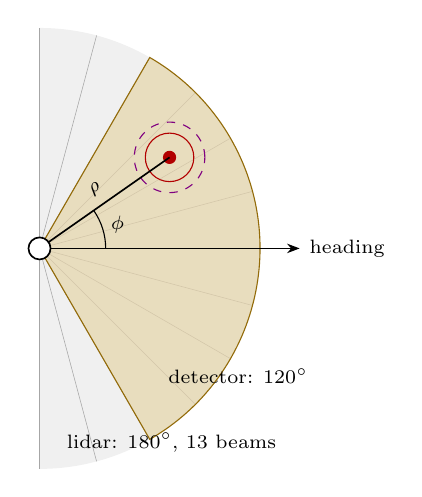
\begin{tikzpicture}[scale=0.56, font=\scriptsize]
        % lidar half-disc (180 deg, 5 m) and its 13 beams
        \fill[black!6] (0,0) -- (0,-5) arc[start angle=-90, end angle=90, radius=5] -- cycle;
        \foreach \a in {-90,-75,...,90}
            \draw[black!35, very thin] (0,0) -- (\a:5);
        % detector cone (120 deg, 5 m)
        \fill[CoverGold!35, opacity=0.7] (0,0) -- (-60:5) arc[start angle=-60, end angle=60, radius=5] -- cycle;
        \draw[CoverGold!80!black] (0,0) -- (-60:5) arc[start angle=-60, end angle=60, radius=5] -- cycle;
        % heading, obstacle, range and bearing
        \draw[-{Stealth[length=1.6mm]}, semithick] (0,0) -- (0:5.9) node[right] {heading};
        \fill[red!70!black] (35:3.6) circle[radius=0.15];
        \draw[red!70!black] (35:3.6) circle[radius=0.55];
        \draw[violet, dashed] (35:3.6) circle[radius=0.8];
        \draw[semithick] (0,0) -- node[above, sloped] {$\rho$} (35:3.6);
        \draw (0:1.5) arc[start angle=0, end angle=35, radius=1.5];
        \node at (17:1.85) {$\phi$};
        % vehicle
        \fill[white] (0,0) circle[radius=0.25];  \draw[semithick] (0,0) circle[radius=0.25];
        \node[align=left, anchor=west] at (0.4,-4.4) {lidar: $180^{\circ}$, 13 beams};
        \node[align=left, anchor=west] at (2.7,-2.9) {detector: $120^{\circ}$};
    \end{tikzpicture}
    \caption{Sensing geometry to scale. An obstacle is shown with its
    clearance ring (solid, $0.40$~m from its surface) and its keep-out
    (dashed, $0.8$~m from its centre).}
    \label{fig:sensing}
\end{figure}

\subsection{Integration with the Guidance Subsystem}
The two layers meet guidance at different points
(Fig.~\ref{fig:architecture}). The re-planner acts on the \emph{input} of guidance:
it replaces the path that guidance follows, and guidance continues with
the same logic on the new path. No mode switch is needed, and the
waypoints are never changed. The reactive layer acts on the
\emph{output} of guidance: it sits between guidance and the controller and modifies
the heading command and the speed.

The reactive layer also hands control back without a switch. When no
obstacle is within reach, its obstacle repulsion is zero and its output
is the guidance heading, filtered and adjusted only by any wall
repulsion. Near a waypoint the reach shrinks to the distance to the
waypoint, though never below $0.7$~m, the lidar wall reach likewise
shrinks from $1.2$~m to no less than $0.5$~m, and the tangential term
fades in proportion, so an obstacle beside a waypoint cannot hold the vehicle
away from it.

\subsection{Limitations}
\textit{Field of view.} An obstacle is known only once it has been
inside the $120^{\circ}$, $5$~m cone, so one just around a corner is
detected late and leaves the reactive layer little room.
\textit{Static obstacles.} A remembered obstacle is never forgotten and
its position is averaged, so obstacles are assumed not to move.
\textit{Estimate error.} Obstacle positions inherit the error of the
state estimate. The margins are sized against its measured
distribution (Section~\ref{sec:estimator}) but are fixed; they do not
shrink or grow with the filter's covariance during a mission. \textit{Local minima.} The reactive layer can stall where
repulsion balances attraction, for example in a gap narrower than the
keep-out; re-planning removes most such cases by routing round the open
side. \textit{Computation.} A re-plan took $0.22$~s to compute on
average and up to $0.92$~s over the $25$ missions of
Section~\ref{sec:results}. The simulation clock waits for it, so it is
not counted in the mission time; a real vehicle would travel up to
about $0.9$~m on the old path first.

% ============================================================
% GUIDANCE SYSTEM AND PART A REUSE  (Requirement 4d)
% ============================================================
\section{Guidance System}
\label{sec:guidance}

\subsection{Subsystems Reused from Part A}
All four Part~A subsystems were carried into Part~B
(Table~\ref{tab:reuse}). They are described in the Part~A reports
\cite{partA_est, partA_group}; only the changes are given here.

\begin{table}[!t]
    \centering
    \caption{Part A Subsystems Reused in Part B}
    \label{tab:reuse}
    \footnotesize
    \begin{tabularx}{\linewidth}{@{}l c >{\raggedright\arraybackslash}X@{}}
        \toprule
        \textbf{Subsystem} & \textbf{Reused} & \textbf{Modification} \\
        \midrule
        State estimator   & Yes    & Same seven-state linear Kalman filter at $100$~Hz. Each pose sample is used in one update, on the step it arrives. $R$ and $Q$ recalibrated from the measured noise (Section~\ref{sec:estimator}). \\
        Waypoint guidance & Partly & Capture logic kept. Straight-line tracking replaced by following the planned path. \\
        Controller        & Yes    & Same structure. Speed limit halved to $1.0$~m/s; speed also scaled by the avoidance layer. \\
        Waypoint ordering & Yes    & Same ant colony optimiser. Cost is A* path length; five waypoints. \\
        \bottomrule
    \end{tabularx}
\end{table}

\subsection{State Estimator and Noise Characterisation}
\label{sec:estimator}
Every other subsystem acts on the estimate $\hat{\mathbf{x}}$, and the
obstacle positions are built from it (Eq.~\eqref{eq:detection}), so its
error sets the margins used throughout this report. The estimator is
the linear Kalman filter of Part~A \cite{partA_est}, run at $100$~Hz on
the state $\mathbf{x} = [p_{x}\ p_{y}\ \theta\ v\ \omega\ v_{x}\ v_{y}]^{\top}$.
Position integrates the Cartesian velocity and heading integrates the
turn rate, so the model is linear:
\begin{equation}
    \mathbf{x}_{k+1} = A\mathbf{x}_{k} + \mathbf{w}_{k}, \qquad
    \mathbf{z}_{k} = H\mathbf{x}_{k} + \mathbf{n}_{k},
    \label{eq:kf}
\end{equation}
where $A$ adds $\Delta t\,v_{x}$, $\Delta t\,v_{y}$ and $\Delta t\,\omega$
to $p_{x}$, $p_{y}$ and $\theta$, and $H$ selects the measured pose and
speed, $\mathbf{z} = [x\ y\ \theta\ v]^{\top}$. The velocity and
turn-rate states are random walks: a white disturbance of intensity $q$
entering a rate gives, for each (position, rate) pair,
\begin{equation}
\begin{aligned}
    Q_{\text{pair}} &= q\begin{bmatrix} \Delta t^{3}/3 & \Delta t^{2}/2 \\ \Delta t^{2}/2 & \Delta t \end{bmatrix}, \\
    R &= \operatorname{diag}(\sigma_{xy}^{2}, \sigma_{xy}^{2}, \sigma_{\theta}^{2}, \sigma_{v}^{2}).
\end{aligned}
\label{eq:kfnoise}
\end{equation}
The pose arrives at $20$~Hz. Each sample is used in one full update on
the step it arrives; on the steps between, only the speed is fused, so a
held sample is never counted twice. The covariance is updated in Joseph
form.

\textbf{Noise characterisation.} $R$ must describe the noise already
present in the simulator's signals. Part~A set it from the project
specification, variances of $0.1$~m$^{2}$ in position and $2$~deg$^{2}$
in heading, which matched the raw errors measured there, $0.32$~m and
$1.4^{\circ}$ \cite{partA_est}. That $R$ was carried into Part~B. The
Part~B model also outputs the vehicle pose before noise is added, so
the noise can be measured directly as the measured minus the noise-free
pose. Over the $25$ missions of Section~\ref{sec:results}
(Table~\ref{tab:noise}) it is zero-mean, uncorrelated between axes and
Gaussian in shape, with a standard deviation of $0.10$~m per axis and
$1.96^{\circ}$ in heading. The
Part~B simulator is therefore three times less noisy in position than
Part~A and somewhat noisier in heading, and the carried-over $R$ was
ten times too large in position. Consecutive samples are correlated ($0.5$) and samples
$0.1$~s apart are not; the filter treats every $20$~Hz sample as
independent, which slightly overstates the information it receives.

\begin{table}[!t]
    \centering
    \caption{Measured Sensor Noise, 25 Missions}
    \label{tab:noise}
    \footnotesize
    \begin{tabularx}{\columnwidth}{@{}X c c c@{}}
        \toprule
        & $x$ & $y$ & $\theta$ \\
        \midrule
        Mean                           & $-0.001$ m & $-0.001$ m & $-0.06^{\circ}$ \\
        Standard deviation             & 0.100 m & 0.097 m & $1.96^{\circ}$ \\
        Autocorrelation, 0.05 s / 0.10 s & 0.50 / 0.00 & 0.52 / 0.03 & 0.51 / 0.02 \\
        Kurtosis (Gaussian: 3)         & 3.22 & 2.97 & 3.07 \\
        \midrule
        \multicolumn{4}{@{}l}{Correlation between $x$ and $y$: $0.02$; \ $59\,624$ pose samples at $20$~Hz} \\
        \multicolumn{4}{@{}l}{Forward speed: mean $-0.008$~m/s, standard deviation $0.105$~m/s} \\
        \bottomrule
    \end{tabularx}
\end{table}

The speed noise was measured the same way, against the speed
differenced from the noise-free pose. Its standard deviation,
$0.105$~m/s, confirms the $\sigma_{v} = 0.1$~m/s carried over from
Part~A; its correlation in time cannot be resolved, because the
reference speed is itself derived from the $20$~Hz pose.
$R$ was set to the measured values, $\sigma_{xy} = 0.10$~m and
$\sigma_{\theta} = 2^{\circ}$, with $\sigma_{v} = 0.1$~m/s unchanged.
The Kalman gain depends on the ratio of $Q$ to $R$, so the velocity
intensity was lowered with it, from $0.5$ to $0.05$~m$^{2}$/s$^{3}$, with
$q_{\omega} = 5$~rad$^{2}$/s$^{3}$. Both settings were chosen by
replaying the filter offline on the logged measurements of missions
$1$ to $8$ over $60$ combinations of $\sigma_{xy}$, $q_{v_{x}, v_{y}}$
and $q_{\omega}$, scored against the noise-free pose. Accuracy is flat
near the optimum: the old and new settings both give $0.079$~m RMS
position error, against $0.078$~m for the best combination tested. What
the recalibration fixes is consistency. A consistent filter has a mean
normalised innovation squared (NIS) equal to the pose dimension, $3$;
the old $R$ gave $0.85$, a filter that overstates its own uncertainty,
and the new one gives $2.5$. Covariance calibration was the main
weakness identified in Part~A \cite{partA_est}. The filter reduces the planar position error
from $0.139$~m RMS in the raw measurement to $0.079$~m, and $99$\% of
its errors are below $0.18$~m. That value is what the $0.20$~m tracking
margin of Section~\ref{sec:planning} and the $0.25$~m obstacle margin of
Section~\ref{sec:avoidance} are sized against. In closed loop on missions
$1$ to $8$ (with the earlier $0.8$~m capture radius), the recalibrated filter also raised the worst true
clearance slightly, from $0.57$ to $0.59$~m to an obstacle and from
$0.63$ to $0.66$~m to a wall.

\subsection{Modifications for Part B}
\textbf{Path following.} In Part~A no wall stood between waypoints.
Here the straight line to a waypoint may pass through a wall, so
guidance follows the planned path, a list of points about $0.1$~m
apart. Guidance keeps an index $k$ into the list and steers at point
$\mathbf{p}_{k}$:
\begin{equation}
    \theta_{\text{cmd}} = \operatorname{atan2}\!\left(p_{k,y} - \hat{y},\ p_{k,x} - \hat{x}\right).
    \label{eq:guidance}
\end{equation}
The index advances whenever the vehicle is within $1.0$~m of
$\mathbf{p}_{k}$, so the target stays about $1.0$~m ahead on the path.

\textbf{Waypoint capture.} The index may not pass the point where the
current waypoint lies on the path, so the vehicle cannot skip a waypoint
by following the path past it. A waypoint is captured within
$r_{c} = 0.4$~m. The last one uses $0.10$~m; on its final approach the
vehicle steers directly at it, and on capture guidance stops the
simulation so that the mission ends on the waypoint.

\textbf{Path replacement.} When the re-planner publishes a new path,
guidance adopts it on the next step. If the leg being driven was
re-planned, the index restarts at the beginning of the new leg, which
is the vehicle's own position at the time of re-planning.

\textbf{Controller.} The turn rate is proportional to the heading error
$e_{\theta} = \theta_{\text{safe}} - \hat{\theta}$, and the speed to the
distance to the waypoint, reduced in turns and near obstacles:
\begin{equation}
    \omega = K_{\theta}\,e_{\theta}, \qquad
    v = K_{d}\,d_{\text{wp}}\cos e_{\theta}\; v_{\text{scale}}.
    \label{eq:controller}
\end{equation}
The turn rate is limited to $\omega_{\max} = 2\pi/5$~rad/s and
$K_{d}\,d_{\text{wp}}$ to $v_{\max} = 1.0$~m/s, and the factor
$\cos e_{\theta}$ is kept between $0.1$ and $1$. The gains are
$K_{\theta} = 1.0$~s$^{-1}$ and $K_{d} = 0.75$~s$^{-1}$. The speed limit
is the main trade-off between mission time and safety and is examined
with the other results in Section~\ref{sec:results}.

% ============================================================
% RESULTS
% ============================================================
\section{Results}
\label{sec:results}

The system was evaluated on $25$ random missions, generated from
seeds $1$ to $25$ so that they can be repeated. Mission time excludes
planning and re-planning, during which the simulation clock is stopped.
Ground truth is the vehicle pose before the simulator adds measurement
noise (Section~\ref{sec:estimator}). Clearance, cross-track error and
closest approach are measured from it. Clearance by the state estimate,
which is what the vehicle itself believed, is given for comparison.
Clearance is measured from the vehicle's centre to a wall face or an
obstacle's surface and must be at least $0.40$~m.

\begin{table}[!t]
    \centering
    \caption{Results over 25 Random Missions}
    \label{tab:results}
    \footnotesize
    \begin{tabularx}{\columnwidth}{@{}X c c c@{}}
        \toprule
        \textbf{Metric} & \textbf{Mean} & \textbf{Min} & \textbf{Max} \\
        \midrule
        Missions completed                    & \multicolumn{3}{c}{25 of 25} \\
        Mission time (s)                      & 122.9 & 78.2 & 175.3 \\
        Planned path length (m)               & 107.6 & 66.6 & 157.3 \\
        Min.\ obstacle clearance (m)          & 0.72 & 0.58 & 1.01 \\
        Min.\ wall clearance (m)              & 0.76 & 0.65 & 0.88 \\
        \quad by estimate: obstacle (m)       & 0.66 & 0.44 & 0.94 \\
        \quad by estimate: wall (m)           & 0.68 & 0.59 & 0.82 \\
        Position error of estimate, RMS (m)   & 0.079 & 0.077 & 0.081 \\
        Capture error, waypoints 1--4 (m)     & 0.39 & 0.38 & 0.40 \\
        Capture error, final waypoint (m)     & 0.094 & 0.062 & 0.100 \\
        Final stop, true distance (m)         & 0.14 & 0.05 & 0.22 \\
        Closest approach, waypoints 1--4 (m)  & 0.12 & 0.05 & 0.23 \\
        RMS cross-track error (m)             & 0.16 & 0.14 & 0.18 \\
        Max.\ cross-track error (m)           & 0.43 & 0.36 & 0.49 \\
        Re-plans per mission                  & 3.2 & 1 & 6 \\
        Re-plan computation (s)               & 0.20 & 0.12 & 0.65 \\
        Obstacle repulsion active (s)         & 0.36 & 0 & 1.61 \\
        Wall repulsion active (s)             & 9.1 & 2.8 & 17.2 \\
        \bottomrule
    \end{tabularx}
\end{table}

\textbf{Completion and time.} All $25$ missions captured every waypoint
in order (Table~\ref{tab:results}). The mean mission took $123$~s for a
$108$~m planned path. The vehicle drove $111$~m, $3.0$\% further, which
is the cost of the detours, of tracking error and of turning onto each
waypoint, at a mean speed of $0.90$~m/s against the $1.0$~m/s limit. By
its estimate the vehicle captured the last waypoint within $0.10$~m in
every mission. By the true pose it stopped $0.14$~m from it on average
and never more than $0.22$~m away; the difference is the estimate error
at the moment of capture. Figure~\ref{fig:mission} shows one mission.

\begin{figure}[!t]
    \centering
    \reportfig{fig_mission.png}
    \caption{Mission 9 as driven, by the true pose. Diamonds mark where
    the path was re-planned.}
    \label{fig:mission}
\end{figure}

\textbf{Clearance.} No mission breached the required clearance
(Fig.~\ref{fig:batch}). The closest true pass was $0.58$~m from an
obstacle, in mission~23, and $0.65$~m from a wall, in mission~14, a
margin of at least $0.18$~m in every mission. The vehicle's own
estimate never put it inside the limit either: its closest estimated
pass was $0.44$~m from an obstacle, in mission~9, where the true
clearance was $0.58$~m. The estimate can place the vehicle up to
$0.14$~m closer to an obstacle than it really is, and this is why the
margins of Sections~\ref{sec:planning} and~\ref{sec:avoidance} are
sized against the measured estimate error rather than against zero.

\begin{figure*}[!t]
    \centering
    \reportfig[0.9\textwidth]{fig_batch.png}
    \caption{Minimum true clearance (left) and mission time with number
    of re-plans (right) for each of the $25$ missions.}
    \label{fig:batch}
\end{figure*}

\textbf{Avoidance layers.} The path was re-planned between one and six
times in every mission. Each re-plan took $0.20$~s to compute on
average and $0.65$~s at most. The obstacle repulsion of the reactive
layer acted in $14$ of the $25$ missions, for $0.36$~s per mission on
average and never for more than $1.61$~s. The wall repulsion acted in
every mission, for $9.1$~s on average, mostly as a light correction in
doorways and narrow corridors. With the re-planner switched off,
six of missions $1$ to $8$ breached the obstacle clearance, the worst
passing $0.27$~m from an obstacle, with the reactive layer acting for
$4.9$~s per mission. At its backup tuning the reactive layer cannot keep the
clearance alone; re-planning is what provides it.

\textbf{Tracking and capture.} The cross-track error, measured from the
true pose against the path that was active at each instant, had an RMS
of $0.16$~m and a largest value of $0.49$~m (Fig.~\ref{fig:timeline}).
The peaks exceed the $0.20$~m added to the wall inflation; it is the
soft clearance, which keeps the path about $0.9$~m from walls wherever
there is room, that absorbs them. Waypoints $1$ to $4$ are captured on
entering a $0.4$~m capture radius, so their capture error equals the
radius by design. The path runs through each waypoint, so the vehicle
carries on past it after capture: its true path passed within $0.12$~m
of them on average and never more than $0.23$~m away.

\begin{figure}[!tb]
    \centering
    \reportfig{fig_timeline.png}
    \caption{True clearance and cross-track error in mission 9. Dotted
    lines mark the two re-plans.}
    \label{fig:timeline}
\end{figure}

\textbf{Speed and capture radius.} Table~\ref{tab:sweep} repeats
missions $1$ to $8$ with one parameter changed at a time. Raising the
speed limit to $1.5$~m/s cut the mission time by $23$\%, but one
mission passed $0.37$~m from an obstacle, and at $2.0$~m/s one mission
breached the clearance again. One cause is known: the paths are planned
for a turn radius of $1.0$~m, but at these speeds the tightest turn the
vehicle can hold grows to $1.2$~m and $1.6$~m, so it can no longer
follow the planned curves, and the RMS cross-track error rises from
$0.17$~m to $0.30$~m and $0.41$~m. A limit of $1.0$~m/s was therefore
the fastest of the three tested that kept the clearance, with no other
parameter re-tuned. Doubling the capture radius to $0.8$~m saved
$3.6$\% in time with no loss of clearance, but the vehicle then passed
the intermediate waypoints $0.35$~m away on average instead of
$0.13$~m. The $0.4$~m radius was chosen so that every waypoint is
visibly visited, at a small cost in time.

\begin{table}[!t]
    \centering
    \caption{Effect of Speed Limit (m/s) and Capture Radius (m), Missions 1--8, by the True Pose}
    \label{tab:sweep}
    \footnotesize
    \begin{tabularx}{\columnwidth}{@{}X c c c c@{}}
        \toprule
        & & $v_{\max}$ & $v_{\max}$ & $r_{c}$ \\
        & \textbf{Base} & \textbf{1.5} & \textbf{2.0} & \textbf{0.8} \\
        \midrule
        Mean mission time (s)          & 117.9 & 90.6 & 79.4 & 113.7 \\
        Worst wall clearance (m)       & 0.68 & 0.54 & 0.42 & 0.66 \\
        Worst obstacle clearance (m)   & 0.59 & 0.37 & 0.35 & 0.59 \\
        Missions below $0.40$~m        & 0 & 1 & 1 & 0 \\
        RMS cross-track error (m)      & 0.17 & 0.30 & 0.41 & 0.16 \\
        Closest approach (m)           & 0.13 & 0.10 & 0.07 & 0.35 \\
        \bottomrule
    \end{tabularx}
\end{table}

% ============================================================
% CONCLUSION
% ============================================================
\section{Conclusion}
\label{sec:conclusion}

This report presented a navigation system that takes a ground robot
through five random waypoints in a walled arena containing obstacles it
can only discover with its own sensors. The mission is planned on the
known walls: ant colony optimisation orders the waypoints by driving
distance, A* routes each leg on a map inflated for clearance, and
particle swarm optimisation smooths each leg towards the vehicle's
turning limit. During the mission, detected obstacles are remembered
and the remaining path is re-planned around them, with a reactive
potential field as a close-range backup. The Part~A estimator,
controller and waypoint optimiser were reused, and guidance was
extended to follow a path that can change during the mission.

Over $25$ random missions the vehicle captured every waypoint, passing
each within $0.23$~m, and, by the simulator's noise-free pose, never
came closer than $0.58$~m to an obstacle or $0.65$~m to a wall, a
margin of at least $0.18$~m over the required $0.40$~m. Re-planning is
what kept the obstacle clearance: with it switched off, six of eight
test missions breached it. Logging the noise-free pose also allowed the
sensor noise to be measured rather than assumed. It is zero-mean and
Gaussian with a standard deviation of $0.10$~m and $2^{\circ}$, and
recalibrating the Kalman filter to it made the filter consistent
without loss of accuracy. A mission took $123$~s on average, and of
the three speed limits tested, $1.0$~m/s was the fastest that kept the
clearance.

The main limitation is the trade between speed and margin. At
$1.5$~m/s the mission was $23$\% faster but one test mission breached
the clearance, because the vehicle cannot follow curves planned for a
$1.0$~m turn radius at that speed, and its own estimate can be over
$0.1$~m from the truth near an obstacle. Planning for a turn radius
that grows with the speed limit, and margins that grow with the
estimator's uncertainty, would allow a faster mission without losing
the margin. Two further limits apply outside simulation: obstacles are
assumed static, and each re-plan takes up to $0.65$~s that the
simulation does not charge for. An incremental planner such as D* Lite
\cite{koenig2002}, which repairs the previous search instead of
repeating it, would address the second.

% ============================================================
% REFERENCES
% ============================================================
\section*{References}
\addcontentsline{toc}{section}{References}

% Stops LaTeX printing its own large "Bibliography" heading.
% Entries are in order of first citation.
\begingroup
\renewcommand{\chapter}[2]{}
\begin{thebibliography}{99}

\bibitem{sanchez2021}
J. R. S\'{a}nchez-Ib\'{a}\~{n}ez, C. J. P\'{e}rez-del-Pulgar and A. Garc\'{i}a-Cerezo, ``Path planning for autonomous mobile robots: A review,'' \textit{Sensors}, vol. 21, no. 23, art. 7898, 2021.

\bibitem{partA_est}
C. Masere, ``Ground-vehicle state estimation: Linear Kalman filtering for waypoint guidance and control,'' EGH446 Major Project Part~A report, Queensland Univ. Technol., Brisbane, Australia, Sep. 2026.

\bibitem{partA_group}
J. Menzies and B. Carkeet, EGH446 Major Project Part~A individual reports, Queensland Univ. Technol., Brisbane, Australia, Sep. 2026.

\bibitem{shami2022}
T. M. Shami, A. A. El-Saleh, M. Alswaitti, Q. Al-Tashi, M. A. Summakieh and S. Mirjalili, ``Particle swarm optimization: A comprehensive survey,'' \textit{IEEE Access}, vol. 10, pp. 10031--10061, 2022.

\bibitem{blum2024}
C. Blum, ``Ant colony optimization: A bibliometric review,'' \textit{Phys. Life Rev.}, vol. 51, pp. 87--95, 2024.

\bibitem{szczepanski2022}
R. Szczepanski, T. Tarczewski and K. Erwinski, ``Energy efficient local path planning algorithm based on predictive artificial potential field,'' \textit{IEEE Access}, vol. 10, pp. 39729--39742, 2022.

\bibitem{urrea2021}
C. Urrea and R. Agramonte, ``Kalman filter: Historical overview and review of its use in robotics 60 years after its creation,'' \textit{J. Sensors}, vol. 2021, art. 9674015, 2021.

\end{thebibliography}
\endgroup



\end{document}
